\documentclass[tikz,border=9pt]{standalone}
\usepackage{amsmath,amssymb}
\usetikzlibrary{arrows.meta,positioning,calc}
\begin{document}
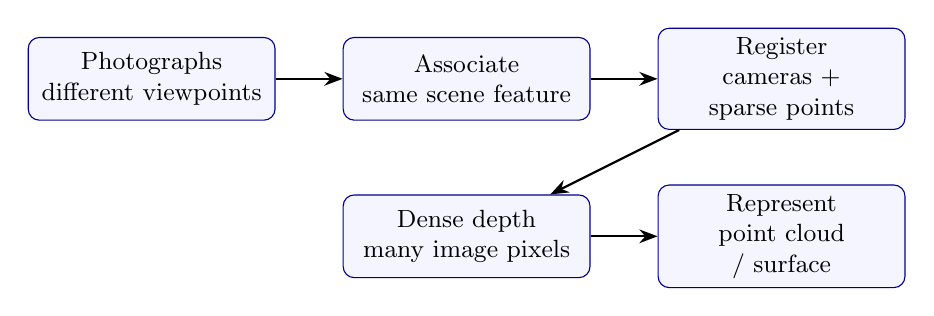
\begin{tikzpicture}[font=\small,arr/.style={-{Stealth},thick},box/.style={draw=blue!55!black,rounded corners,fill=blue!4,align=center,text width=2.9cm,minimum height=1.05cm}]

\node[box] (a) at (0,0) {Photographs\\different viewpoints};
\node[box] (b) at (4,0) {Associate\\same scene feature};
\node[box] (c) at (8,0) {Register\\cameras + sparse points};
\node[box] (d) at (4,-2) {Dense depth\\many image pixels};
\node[box] (e) at (8,-2) {Represent\\point cloud / surface};
\draw[arr] (a)--(b);\draw[arr] (b)--(c);\draw[arr] (c)--(d);\draw[arr] (d)--(e);

\end{tikzpicture}
\end{document}
